\section{Data and theory}
\label{sec:theory}

In this work, the photon
content of the proton $\gamma(x,Q^2)$ is extracted from a PDF analysis based
on the legacy inclusive structure function data combination from HERA~\cite{Abramowicz:2015mha}
supplemented by the ATLAS measurements of the high-mass Drell-Yan process
at $\sqrt{s}=8$ TeV~\cite{Aad:2016zzw}.
%
The HERA structure functions are the backbone of all
recent PDF fits, providing information on the quark/antiquark and gluon content of 
the proton, while the high-mass Drell-Yan data provide
direct sensitivity to the photon PDF.
%
Indeed, dilepton production at the Born level can arise  from either quark-antiquark $s$-channel
scattering or from photon-photon $t$-channel scattering mediated by a lepton,
as shown in Fig.~\ref{fig:photoninduced}.

%%%%%%%%%%%%%%%%%%%%%%%%%%%%%%%%%%%%%%%%%%%%%%%%%%%%%%%%%%%%%%%%
\begin{figure}[t]
  \begin{center}
    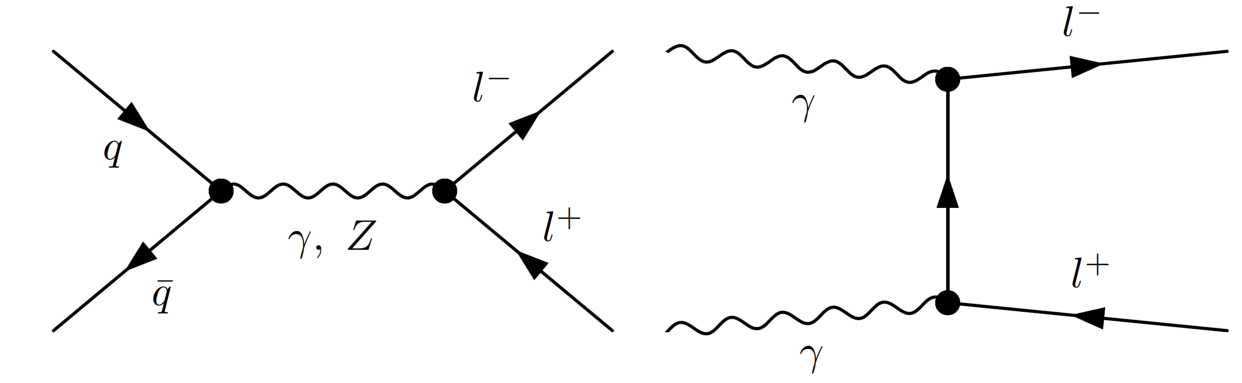
\includegraphics[width=15cm]{figs/photoninduced.pdf}
    \end{center}
  \caption{Two of the processes that contribute to lepton-pair
  production at hadron colliders at the Born level.}
\label{fig:photoninduced}
\end{figure}
%%%%%%%%%%%%%%%%%%%%%%%%%%%%%%%%%%%%%%%%%%%%%%%%%%%%%%%%%%%%%%%%

Deep-inelastic structure functions and PDF evolution is performed
with the program {\tt APFEL}~\cite{Bertone:2013vaa}, whic is accurate currently 
up to NNLO for the QCD corrections and up to NLO for the QED corrections, as described in appendix~\ref{sec:appendixAPFEL}.
%
To be precise, this means that the DGLAP evolution equations \cite{XXXXXX} are solved including
the splitting functions $P(\alpha_s,\alpha)$ up to $\mathcal{O}\lp \alpha_s^3\rp$ in the QCD
coupling and up to $\mathcal{O}\lp \alpha_s\alpha\rp$ in the QED coupling,
and that DIS coefficient functions include corrections up to $\mathcal{O}\lp \alpha_s^2\rp$
in QCD and up to $\mathcal{O}\lp \alpha^2\rp$ in QED.

Heavy quark (charm and bottom) mass effects in DIS structure functions are taken into account
using the FONLL-B(C) general-mass scheme~\cite{Forte:2010ta}
for the NLO (NNLO) fits.
%
As for the numerical values of the heavy quark masses in the pole scheme,
we take  $m_c=1.47~$GeV and $m_b=4.5~$GeV, consistent with the latest
PDG averages~\cite{Agashe:2014kda}.
%
%With the same motivation, 
The coupling constants are chosen to be  $\alpha_s(m_Z)=0.118$ and 
$\alpha(m_Z)=1/127$, according to PDG.
%%%%% Can we put this somewhere else? 
Let us recall that heavy quark structure functions with running masses
are also implemented in {\tt APFEL}~\cite{Bertone:2016ywq},
though their use should not lead to any difference for the determination of the photon PDF.
%
The charm PDF is generated perturbatively from light quarks and gluons using
the DGLAP equations.

For the calculation of high-mass Drell-Yan cross-sections,
we use the {\tt MadGraph5{\_}aMC@NLO}~\cite{Alwall:2014hca} program  v2.4.3,
which includes the contribution from photon initiated corrections,
and interfaced to {\tt APPLgrid}~\cite{Carli:2010rw} v1.4.7
and {\tt aMCfast}~\cite{amcfast} v1.3).
%
A tailored version of  {\tt APPLgrid} was used, allowing to account for
the contribution of photon-initiated processes.
%
The calculation is performed in the $n_f=5$ scheme neglecting the masses of the charm
and bottom quarks in the matrix elements, as appropriate for a high-scale processes
with $Q \gg m_Z$.

The ATLAS high-mass Drell-Yan 8 TeV measurements include both the one-dimensional (1D)
invariant mass distribution, $d\sigma/dm_{ll}$, as well as double-differential (2D)
distributions in $m_{ll}$ and $y_{ll}$, the rapidity of the dilepton pair,
$d^{2}\sigma/dm_{ll}d|y_{ll}|$, and in $m_{ll}$ and $\Delta\eta_{ll}$,
  the difference in 
  pseudorapidity between the lepton pair, $d^{2}\sigma/dm_{ll}\Delta\eta_{ll}$.
  %
  For the invariant mass 
  distribution, there are 12 bins between 116 GeV and 1.5 TeV; and for both of the 
 the two-dimensional distributions, there are five different histograms, each one for a different invariant
 mass range, from the lowest bin
 with 116 GeV < $m_{ll}$ < 150 GeV to the highest bin with 500 GeV < $m_{ll}$ < 1500 GeV.
 %
 The first three (last two) $m_{ll}$ bins are divided into 12 (6) bins with fixed
 width, extending up to 2.4 and 3.0 for the  $|y_{ll}^{mim}|$ and $|\Delta\eta_{ll}|$ distributions
 respectively.
 %
 In Sect.~\ref{sec:results} we compare the impact on the photon PDF of fitting either
 the 1D distributions or one of the two 2D distributions.

 In the theoretical calculations of the Drell-Yan cross-section we use
 dynamical  renormalization $\mu_{R}$ and factorization $\mu_{R}$ scales,
 both set equal to the invariant mass  $m_{ll}$ of each bin.
 %
  The {\tt MadGraph5{\_}aMC@NLO} theoretical predictions for these measurements
  follow the analysis cuts, including $m_{ll}\ge 116$ GeV,
  $\eta_l\le 2.5$, $p_T^l \ge 40~(30)$ for the leading (sub-leading) lepton.
 %
 The {\tt MadGraph5{\_}aMC@NLO} calculation used in this work were benchmarked with
 the corresponding  predictions (NLO QCD and LO QED, including photon-induced processes)
 obtained with the {\tt FEWZ} code~\cite{Gavin:2012sy} v3.1, finding agreement at the 1\% level or better
 for both the 1D and the 2D distributions.
 %
 In order to achieve NNLO QCD and NLO EW accuracy in our theoretical calculations, the
 NLO QCD + LO QED {\tt APPLgrids} generated with {\tt MadGraph5{\_}aMC@NLO} as specified
 above have been supplemented by bin-by-bin $K$-factors, defined
 as
 \begin{equation}
  \label{eq:kfactor}
K \equiv\frac{\rm NNLO\  QCD  + NLO\  EW}{\rm NLO\  QCD + LO\  EW} \, ,
 \end{equation}
 using a fixed PDF set, MMHT2014 NNLO~\cite{Harland-Lang:2014zoa}, both in the numerator
 and in the denominator (though NNLO $K$-factors depend very mildly on the
 input PDF set).
 %
 The $K$-factor Eq.~({\ref{eq:kfactor}) has also  been 
computed using
{\tt FEWZ}, with the same settings as
the corresponding NLO computations.
%

In Fig.~\ref{fig:kf} we show these $K$-factors as a function
of the dilepton rapidity $|y_{ll}|$, where each curve corresponds
to a different dilepton invariant mass $m_{ll}$ bin.
%
We observe that the $K$-factors vary between 0.98 and 1.04,
highlighting the fact that
higher-order corrections to the Drell-Yan process are moderate,
in particular at low values of $m_{ll}$ and in the central region.
%
Even at forward rapidities, the $K$-factors modify the NLO result
by at most 3\%.


%%%%%%%%%%%%%%%%%%%%%%%%%%%%%%%%%%%%%%%%%%%%%%%%%%%%%%%%
\begin{figure}[t]
\includegraphics[width=9cm]{figs/kf_2D.pdf}
\caption{The NNLO/NLO $K$-factors, defined
  in  Eq.~(\ref{eq:kfactor}), that allow accounting for
    higher order QCD and EW effects in the PDF fits, as a function
    of the dilepton rapidity $|y_{ll}|$.
    Each curve correspond
  to one of the $m_{ll}$ invariant mass bins.}
\label{fig:kf}
\end{figure}
%%%%%%%%%%%%%%%%%%%%%%%%%%%%%%%%%%%%%%%%%%%%%%%%%%%%%%%%

  
